\chapter{Generazione di numeri pseudo-casuali}
\label{ch:rnd}

Alla base di una qualsivolglia simulazione risiede la centralit\`a del ruolo rivestito dalla riproduzione dell'aleatoriet\`a riscontrabile all'interno dei sistemi reali. Per questo motivo \`e fondamentale valutare e conoscere le entit\`a alle quali si fa riferimento per la generazione di numeri casuali, il cui comportamento incider\`a in maniera rilevante sulla qualit\`a delle simulazioni.

Per la generazione di numeri pseudo-casuali sono stati considerati, in fase di analisi, quattro metodologie alternative, le cui caratteristiche sono riportate all'interno dell'apposita scheda presente nell'interfaccia grafica del simulatore:
\begin{itemize}
\item {\tt java.util.Random}\\
	generatore predefinito dell'environment Java per la generazione di numeri pseudo-casuali.
\item {\tt ran0}\\
	generatore lineare congruenziale di tipo \emph{ran0}, implementato ex-novo.
\item {\tt SecureRandom}\\
	generatore presente all'interno del package {\tt java.security} in grado di generare sequenze pseudo-casuali crittograficamente robuste.
\item {\tt MersenneTwister}\\
	generatore implementato all'interno del progetto Apache che realizza l'algoritmo Matsumoto-Nishimura.
\end{itemize}


\section{Generatori lineari congruenziali}

I generatori lineari congruenziali rappresentano una tra le pi\`u conosciute e sperimentate alternative per la generazione di numeri pseudo-casuali. 

Il meccanismo di generazione \`e definito, ricorsivamente, come:

$$
Z_{i}=(a \cdot Z_{i-1}+c)\mod m
$$

dove:\\
$Z_{i}$ rappresenta l'i-esima istanza generata\\
$m \thickspace(0<m)$		, il modulo\\
$a \thickspace(0<a<m)$		, il ``moltiplicatore''\\
$c \thickspace(0\le c<m)$	, l'incremento\\
$Z_{0}$ il seme della sequenza (seed)\\

Il periodo di un generatore lineare congruenziale \`e al pi\`u pari a $m$\footnote{in questo caso il periodo del generatore \`e detto ``pieno''.}, a patto di rispettare alcuni vincoli:
\begin{itemize}
\item[-] $c$ ed $m$ siano coprimi tra loro
\item[-] $(a-1)$ sia divisibile per tutti i fattori primi di m
\item[-] $(a-1)$ sia multiplo di 4, qualora anche $m$ lo sia
\end{itemize}

Le modalit\`a secondo le quali questo tipo di generatori sono definiti fanno s\`i che essi siano particolarmente apprezzati per la loro leggerezza, vista la necessit\`a di memorizzare le sole variabili di stato per un corretto funzionamento e la semplicit\`a dei calcoli necessari per la generazione. Moltiplicazioni tra interi ed il calcolo del modulo sono infatti operazioni che un moderno microprocessore pu\`o realizzare in maniera molto performante.
Tuttavia esiste correlazione tra i valori generati successivamente, che determina l'impossibilit\`a di utilizzare questo tipo di generatori in ambienti in cui tale correlazione rappresenti un fattore di rischio, come ad esempio in ambito crittografico.

\subsection{Classe {\tt Random}}
\label{sec:rndjava}
La classe {\tt Random}, presente all'interno del package {\tt java.util}, rappresenta lo standard per la generazione di valori pseudo-casuali all'interno dell'environment Java.


\begin{table}[!h]
	\begin{center}
	\begin{tabular}{c|c}
	parametro & valore\\
	\hline
	$m$ & $2^{48}$  \\
	$a$ & $25214903917$  \\
	$c$ & $11$  \\
	\end{tabular}
	\end{center}
	\caption{Parametri del LCG implementato in {\tt java.util.Random}}
	\label{tab:rndjava}
\end{table}

Si tratta di un LCG caratterizzato dai parametri mostrati in tab.\ref{tab:rndjava}
e dotato quindi di un periodo pari a  $2^{48} \thickspace (281,474,976,710,656)$.
Un'istanza della classe {\tt Random} permette di ``prelevare'' valori pseudo-casuali di diverso tipo a seconda delle necessit\`a, mediante l'invocazione parametrizzata del metodo protetto {\tt next()}.

Il seme della sequenza pseudo-casuale, formato da 48 bit, pu\`o essere specificato in modo esplicito all'atto della costruzione ({\tt Random(long seed)}), o acquisito tramite l'invocazione interna del metodo {\tt System.currentTimeMillis()} nel caso in cui si ricorra al costruttore standard.

\subsection{Generatore {\tt ran0}}

Il generatore realizzato ex-novo per il simulatore \`e di tipo lineare congruenziale (\emph{ran0}). Come possibile osservare in tabella \ref{tab:rndcustom}, il parametro $c$ \`e stato posto uguale a $0$: questo caratterizza il generatore come di tipo ``Park-Miller'' (moltiplicativo).

Analogamente a quanto visto nel caso del LCG standard di Java, il generatore pu\`o o meno essere instanziato unitamente ad un seed di partenza. In caso tale parametro venga omesso si ricorrer\`a nuovamente alla chiamata 
{\tt System.currentTimeMillis()} per l'ottenimento di un valore arbitrario da impostare come seed iniziale.

\begin{table}[!h]
	\begin{center}
	\begin{tabular}{c|c}
	parametro & valore\\
	\hline
	$m$ & $2147483647$  \\
	$a$ & $16807$  \\
	$c$ & $0$  \\
	\end{tabular}
	\end{center}
	\caption{Parametri del LCG implementato ex-novo ({\tt RandomProvider})}
	\label{tab:rndcustom}
\end{table}

\subsection{SecureRandom}

La classe {\tt SecureRandom} presente all'interno del package {\tt java.security} estende la classe {\tt Random} discussa in precedenza, e permette la generazione robusta dal punto di vista crittografico di numeri pseudo-casuali attraverso l'agoritmo\footnote{e.g. {\tt ``SHA1PRNG''} che segue le specifiche dello standard IEEE P1363} e l'eventuale provider specificati nella chiamata di instanziamento.

Il seed verr\`a poi automaticamente generato attraverso l'invocazione automatica del metodo {\tt setSeed()}.

\subsection{MersenneTwister}

La classe {\tt MersenneTwister}, sviluppata dal progetto \emph{Apache} e disponibile all'interno del package {\tt commons.math.random.MersenneTwister}, implementa l'algoritmo ideato da Makoto Matsumoto e Takuji Nishimura nel 1996/97. 

Questo generatore \`e caratterizzato da un periodo parcolarmente lungo (pari a $2^{19937}-1$), da una equidistribuzione a 623 dimensioni e da una accuratezza massima pari a 32 bit.

L'algoritmo \`e basato sulla seguente ricorsione lineare:

$$x_{k+n}:=x_{k+m} \oplus (x_{k}^{u}|x_{k+1}^{l})A, (k=0,1,...)$$

per il cui approfondimento si rimanda alla bibliografia \cite{matsumoto}.

\subsection{Analisi tecnica: classe {\tt RandomProvider}}

All'interno della classe {\tt RandomProvider}, oltre al generatore creato ex-novo, vengono gestite tutte le tipologie di generatori disponibili, elencate all'interno dell'{\tt enum Provider}. In particolare all'interno della chiamata per l'instanziamento \`e possibile specificare la tipologia di generatore che si intende utilizzare, permettendo una fruizione del servizio disaccoppiata dalla specifica implementazione scelta.

\section{Analisi del generatore}

Il generatore che si \`e scelto di utilizzare come default per il simulatore \`e quello fornito dalla classe {\tt Random} di Java. Tale scelta \`e stata dettata dalla estrema efficienza computazionale di tale generatore e dalla trascurabile rievanza degli effetti della correlazione per l'applicazione di interesse.

\subsection{Distribuzione uniforme in [0,1]}

Per la valutazione dell'uniformit\`a della distribuzione dei valori generati si \`e deciso di realizzare uno scatter plot. Per la realizzazione di questo grafico \`e necessaria la generazione di $N$ coppie di numeri pseudo-casuali, i quali devono essere generati in modo consecutivo, senza variare il seme dell'algoritmo di generazione. Le coppie generate sono quindi utilizzate come le coordinate $X$ e $Y$ dei punti da mostrare nel grafico. Nel caso pi\`u generale \`e possibile specificare un numero variabile di generazioni che devono essere effettuate per ogni coppia tra la coordinata dell'ascissa e dell'ordinata: nel nostro caso si \`e scelto di usare la generazione immediatamente successiva a quella dell'ascissa. Questo grafico permette di individuare correlazioni evidenti tra i valori o problemi dovuti a parametri critici dell'algoritmo, che si presentano come disposizioni ordinate dei punti del grafico.   In figura \ref{fig:random} si mostra la distribuzione dei valori generati da un'istanza della classe Random: \`e possibile apprezzare il buon livello di dispersione e la discreta uniformit\`a dei punti nella copertura dello spazio.
La sezione del simulatore dedicata all'analisi di generatori di numeri random permette di creare dinamicamente scatter plot per ciascuna delle 4 tipologie di generatori discussi in precedenza.



\begin{figure}[!h]{
	\begin{center}
	   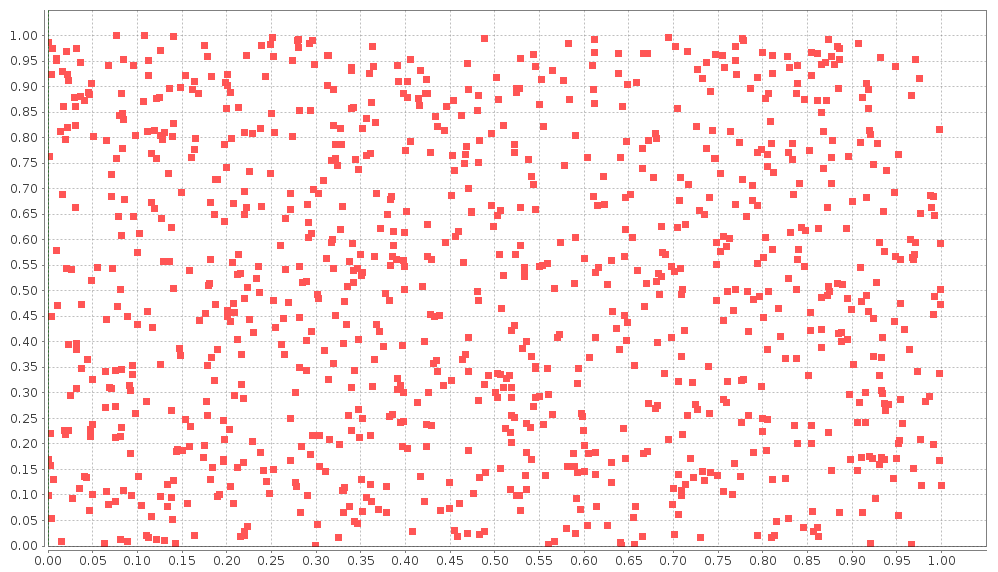
\includegraphics[width=0.95\textwidth]{figures/random.png}
	\end{center}}
	\caption{Distribuzione dei valori generati da {\tt util.Random}}
	\label{fig:random}
\end{figure}


\subsection{Stima del valore medio}

Al fine di permettere un'agevole valutazione visiva del valor medio delle sequenze di numeri pseudo-casuali prodotte si \`e ricorsi ad una serie di generazioni con campioni di dimensione crescente.

\begin{figure}[!h]{
	\begin{center}
	   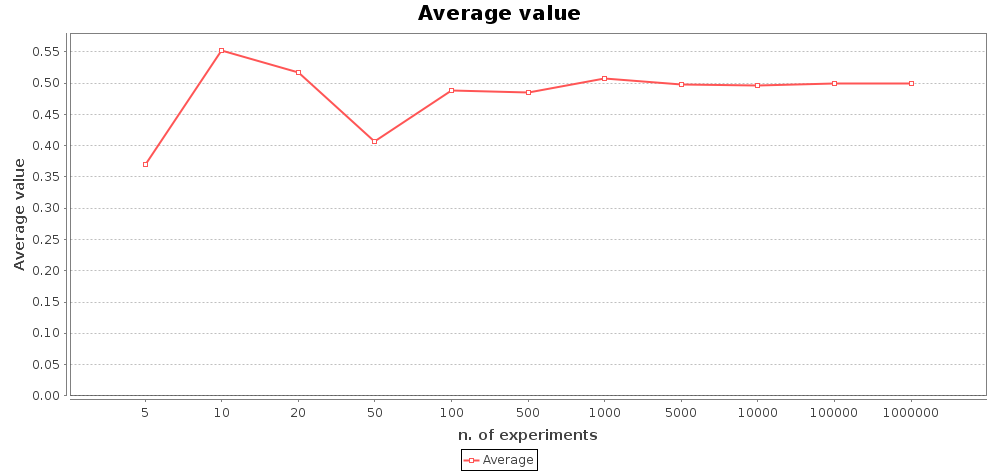
\includegraphics[width=0.95	\textwidth]{figures/average.png}
	\end{center}}
	\caption{Media dei campioni in funzione della numerosit\`a}
	\label{fig:avg}
\end{figure}

In figura \ref{fig:avg} \`e possibile osservare come, all'aumentare della dimensione dei campioni, si abbia una convergenza al valore teorico di $0.5$.
In particolare, gi\`a a partire da qualche migliaio di esperimenti, si pu\`o osservare un'importante grado di aderenza al valore teorico. 

L'andamento della media campionaria presenta sempre ad ogni ripetizione dell'esperienza la stessa tendenza a convergere al valore teorico atteso, con oscillazioni rilevanti presenti esclusivamente in concomitanza ai campioni di piccole dimensioni, come era lecito attendersi.

Anche per l'analisi del valor medio dei numeri pseudo-casuali generati \`e possibile selezionare le varie tipologie di generatori messe a disposizione, ottenendo di volta in volta il relativo grafico.

\subsection{Intervallo di confidenza}

Per la valutazione degli intervalli di confidenza sono state effettuati esperimenti sia al variare del livello di confidenza, sia al variare del numero di campioni. 
Come era lecito aspettarsi, l'intervallo di confidenza mostra un andamento decrescente all'aumentare del numero di campioni presi in considerazione, mentre ha un'andamento crescente all'aumentare del livello di confidenza richiesto.
I grafici ci hanno permesso inoltre di confrontare quantitativamente i valori calcolati dalle funzionalit\`a da noi realizzate con i valori teorici, confermandoci la loro corretta implementazione

\begin{figure}[!h]{
	\begin{center}
	   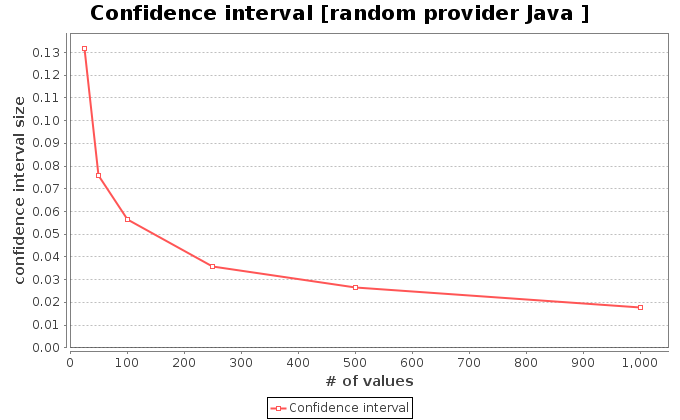
\includegraphics[width=\textwidth]{figures/IDC_1.png}
	\end{center}}
	\caption{Intervallo di confidenza in funzione del numero di campioni}
	\label{fig:idc1}
\end{figure}

In fig.\ref{fig:idc1} e \ref{fig:idc2} \`e possibile osservare l'andamento dell'IDC in funzione del numero di esperimenti svolti e del livello di confidenza, rispettivamente.

\begin{figure}[!h]{
	\begin{center}
	   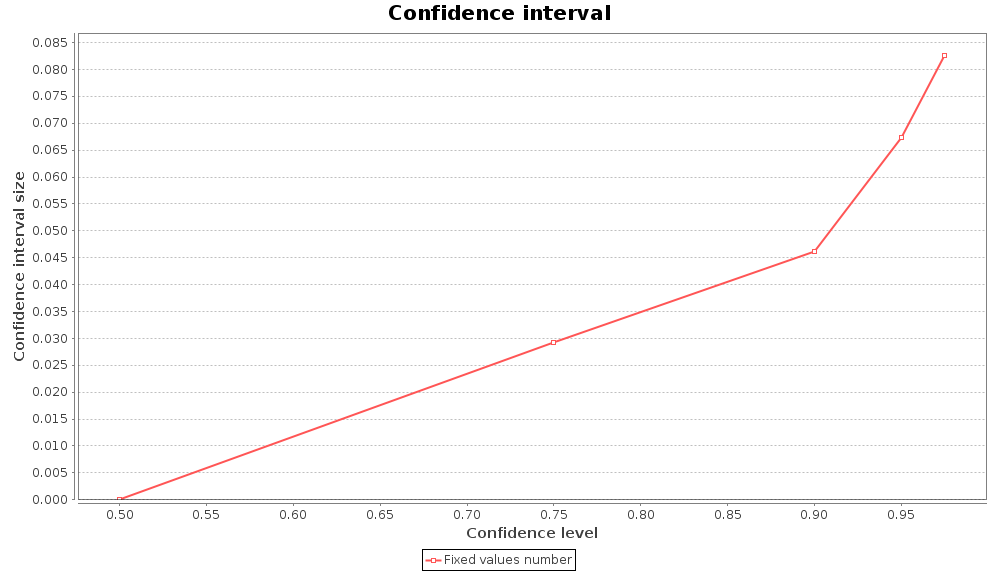
\includegraphics[width=\textwidth]{figures/IDC_2.png}
	\end{center}}
	\caption{Intervallo di confidenza in funzione del livello di confidenza}
	\label{fig:idc2}
\end{figure}

\subsection{Analisi tecnica}

L'esecuzione effettiva delle due possibili tipologie di simulazione per il calcolo dell'intervallo di confidenza (in funzione del numero di run o del livello di confidenza) \`e opera, rispettivamente,  dei metodi:
\begin{itemize}
\item {\tt testConfidenceIntervalWithVariableConfidence(...)} 
\item {\tt testConfidenceIntervalWithVariableRuns(...)}
\end{itemize} 

della classe {\tt SimulationRunners}. All'interno di quest'ultima sono stati infatti raccolti, al fine di ottenere una struttura topologicamente ben organizzata,  i metodi corrispondenti alle varie tipologie di esperimenti messi a disposizione dal simulatore implementato.

All'utente viene data la possibilit\`a di scegliere un generatore di numeri pseudo-casuali tra i quattro esposti al capitolo \ref{ch:rnd}, e di specificare la tipologia di simulazione ed il relativo parametro di riferimento. 

Una volta terminata la parte computazionale, attraverso un apposito metodo della classe {\tt gui.GraphUtils}, viene generato e visualizzato un grafico riportante gli esiti della simulazione.

La classe {\tt GraphUtils} verr\`a in seguito utilizzata per la creazione della totalit\`a dei grafici generati a seguito delle simulazioni, vista la volont\`a di mantenere una strutturazione ben organizzata di classi e package all'interno del progetto.

\subsection{Realizzazione dei grafici}
Per la realizzazione dei grafici relativi alle simulazioni si \`e ricorsi all'utilizzo del tool gratuito \emph{JFreeChart}\footnote{http://www.jfree.org/jfreechart/}, che permette la realizzazione di grafici all'interno dell'invironment Java, oltre a permettere l'esportazione degli stessi in diversi formati di immagine (png).
JFreeChart mette a disposizione numerose tipologie di grafici e diagrammi, consentendo una gamma di personalizzazioni pressoch\'e illimitata.
Si \`e deciso di appoggiarsi a questa libreria poich\'e, implementando il simulatore in Java, si ha l'indubbio vantaggio di poter mostrare i grafici direttamente da codice, senza bisogno di utilizzare tool esterni e senza dover estrarre ed esportare i dati dal simulatore. Inoltre, il framework che la libreria mette a disposizione consente di navigare, ridimensionare, zoomare ed editare i chart tramite interfaccia grafica, consentendoci di ottimizzare la presentazione dei dati in maniera pi\`u rapida.

%\begin{figure}{
%	\begin{center}
%	   \includegraphics[width=\textwidth]{figures/esempi.png}
%	\end{center}}
%	\caption{Tipologie ricorrenti di artefatti: boundary artifacts (B), resource artifacts (R), coordination %%artifacts (C).}
%	\label{fig:esempi}
%\end{figure}

%\begin{table}
%	\begin{center}
%	\begin{tabular}{c|c}
%	Title & $ values $\\
%	\hline
%	10 &  0.5741\\	
%	\end{tabular}
%	\end{center}
%	\caption{Valori medi relativi ai valori generati}.
%	\label{tab:media}e
%\end{table}
